% =============================================================================
% EE302 Final Project (PS9, deliverable D6): MagLev report, Group 22
% Layout: single-column A4 (IEEE two-column made optional by the instructor,
% 2026-11-17); section order follows the instructor's format (Introduction ...
% Precautions, References). Numbers come only from report/numbers.md.
% Compile from this folder:  latexmk -pdf main.tex
% =============================================================================
\documentclass[11pt,a4paper]{article}

\usepackage[T1]{fontenc}
\usepackage{lmodern}
\usepackage[a4paper,margin=2.5cm,headheight=14pt]{geometry}
\usepackage{amsmath,amssymb,amsfonts}
\usepackage{graphicx}
\usepackage{booktabs}
\usepackage{array}
\usepackage{longtable}
\usepackage{tabularx}
\usepackage{multirow}
\usepackage{tikz}
\usetikzlibrary{shapes,arrows.meta,positioning,calc}
\usepackage{siunitx}
\sisetup{detect-all, range-phrase={--}, range-units=single}
\usepackage{float}
\usepackage[font=small,labelfont=bf]{caption}
\usepackage{subcaption}
\usepackage{enumitem}
\usepackage{xcolor}
\usepackage{fancyhdr}
\usepackage{url}
\def\UrlBreaks{\do\/\do\.\do\-\do\_\do\?\do\=\do\&}
\usepackage[hidelinks]{hyperref}

% ------------------------------------------------------------------
% Page style
% ------------------------------------------------------------------
\pagestyle{fancy}
\fancyhf{}
\lhead{\small EE302 Final Project (PS9), Group 22}
\rhead{\small Magnetic Levitation: Robust Control}
\cfoot{\thepage}
\renewcommand{\headrulewidth}{0.4pt}
\setlength{\parskip}{3pt}
\setlist{itemsep=2pt,topsep=3pt}

% ------------------------------------------------------------------
% Helper macros
% ------------------------------------------------------------------
\newcommand{\code}[1]{\texttt{\detokenize{#1}}}
% Status labels (Section 4): M measured, S simulated, D derived, N not obtained, B manual benchmark
\newcommand{\st}[1]{\,\textup{(#1)}}
% Figure box: shows the image if the file exists, otherwise a labelled placeholder.
% usage: \figbox{file}{width}{placeholder height}
\newcommand{\figbox}[3]{%
  \IfFileExists{#1}{\includegraphics[width=#2]{#1}}{%
    \fbox{\parbox[c][#3][c]{\dimexpr#2-2\fboxsep-2\fboxrule\relax}{\centering\footnotesize\textsf{[Insert image]}\\[2pt]\texttt{\detokenize{#1}}}}}}
% One report figure: \repfig{label}{file}{width}{caption}
\newcommand{\repfig}[4]{%
  \begin{figure}[H]\centering\figbox{#2}{#3}{5cm}\caption{#4}\label{fig:#1}\end{figure}}
% Placeholder for text still to be written: \todo{stage}{what goes here}
\newcommand{\todo}[2]{\par\noindent\fcolorbox{orange!80!black}{orange!8}{\parbox{\dimexpr\linewidth-2\fboxsep-2\fboxrule\relax}{\small\textbf{[Stage #1]} #2}}\par}
% Caption obligation from numbers.md (kept visible until the caption is written)
\newcommand{\capnote}[1]{\textcolor{orange!70!black}{[caption must say: #1]}}

\begin{document}

% =============================== COVER PAGE ===============================
\pagenumbering{alph}% title page: unique link anchor
\begin{titlepage}
\thispagestyle{empty}

\begin{center}
{\LARGE\bfseries ROBUST CONTROL DESIGN AND EXPERIMENTAL VALIDATION\\[4pt] OF A MAGNETIC LEVITATION SYSTEM}\\[14pt]
{\large Final Project --- Problem Statement 9}
\end{center}

\vspace{1.4cm}
\noindent
\begin{tabular}{@{}p{3.8cm}l@{}}
Course Code & : EE302 \\[4pt]
Course Name & : Control Systems Laboratory \\[4pt]
Department & : School of Computing and Electrical Engineering \\[4pt]
Institute & : Indian Institute of Technology Mandi \\[4pt]
Course Instructor & : Dr. Yanumula Venkata Karteek \\[4pt]
Teaching Assistant & : \\[4pt]
Date of Experiment & : 12\textsuperscript{th}--16\textsuperscript{th} November, 2026 \\[4pt]
Submission Date & : 17\textsuperscript{th} November, 2026 \\[4pt]
Group Number & : 22 \\
\end{tabular}

\vspace{1.6cm}
\begin{center}
{\bfseries GROUP MEMBER DETAILS}\\[8pt]
\begin{tabular}{@{}clll@{}}
\toprule
S.No. & Name & Roll No. & Signature \\
\midrule
1 & Neil Bakshi & B24344 & \hspace{3cm} \\[8pt]
2 & Ritvik Garg & B24349 & \\[8pt]
3 & Saurabh Gopal & B24352 & \\[8pt]
4 & Snehal Narendra Patil & B24353 & \\[8pt]
\bottomrule
\end{tabular}
\end{center}

\vfill
\begin{center}
August--December 2026
\end{center}

\end{titlepage}

% ================================ ABSTRACT ================================
\pagenumbering{roman}
\begin{abstract}
\todo{F}{Abstract, written last: plant and goal; identified model (force law, coil, delay); cascade design;
robust stability over the uncertainty set (worst $M_s$ above the target, stated); simulation cases; hardware results
(range, kg test, variant D); simulation vs hardware; the stand-proximity effect; what was not obtained.}

\medskip
\noindent\textbf{Keywords:} magnetic levitation, cascade control, robust stability, multiplicative uncertainty,
sensitivity peak, system identification, loop delay, INTECO MLS1EM.
\end{abstract}

\tableofcontents
\listoffigures
\listoftables
\clearpage
\pagenumbering{arabic}

% ============================== 1 INTRODUCTION ==============================
\section{Introduction}
\label{sec:intro}
A magnetic levitation system holds a steel ball in the air below an electromagnet. The pull of the magnet grows as
the ball comes closer, so any small error grows by itself: if the ball rises slightly, the pull increases and lifts
it further; if it drops, the pull weakens and it falls. Without feedback the ball either sticks to the magnet or
falls, which makes the plant \emph{open-loop unstable}. The force also depends nonlinearly on both the gap and the
coil current, the unstable motion is fast (it doubles in about $17$\,ms, Section~\ref{sec:th-lin}), and the
controller acts only through a coil whose current lags the command. A controller must therefore be fast, must work
over a range of operating points, and must tolerate the difference between any model and the real rig.

Problem Statement~9~\cite{ps9} asks for such a controller for the INTECO MLS1EM rig~\cite{mlsmanual}: identify a
linearized operating model, characterize parametric and unstructured uncertainty, design a robust controller that
accommodates operating-point changes, verify stability and robustness in MATLAB/Simulink, and demonstrate stable
levitation on the hardware. Its five requirements (R1--R5) and six deliverables (D1--D6) are listed in
Table~\ref{tab:deliverables} with the parts of this report that answer them.

\begin{table}[H]
\centering
\caption{Problem Statement~9: requirements, deliverables and where they are answered}
\label{tab:deliverables}
\begin{tabularx}{\linewidth}{@{}lXl@{}}
\toprule
Item & Requirement / deliverable & Sections \\
\midrule
R1, D1 & Operating point, linearized model, assumptions, operating range & \ref{sec:th-model}, \ref{sec:th-lin}, \ref{sec:obs-ident}, \ref{sec:obs-unc} \\
R2, D1 & Parametric and unstructured uncertainty, justified by data & \ref{sec:obs-ident}, \ref{sec:obs-unc}, \ref{sec:obs-stand} \\
R3, D3 & Robust control law, design approach, stability and robustness criteria & \ref{sec:th-cascade}, \ref{sec:th-robust}, \ref{sec:obs-design}, \ref{sec:discussion} \\
R4, D2, D4 & Simulink models of the nominal and uncertain cases; margins over the uncertainty range; simulation plots & \ref{sec:scripts}, \ref{sec:obs-robust}, \ref{sec:obs-cases}, App.~\ref{app:scripts} \\
R5, D5 & Hardware implementation, recorded data, simulation versus hardware & \ref{sec:obs-first}--\ref{sec:obs-varD} \\
D6 & Technical report and presentation & this report (presentation separate) \\
\bottomrule
\end{tabularx}
\end{table}

The work was done in three lab sessions (12, 13 and 16 November 2026) with offline analysis between them. It
produced an identified nonlinear model, an uncertainty set built from the measurements, a cascade controller
(an inner coil-current loop inside an outer position loop), a Simulink model run over 77 cases, and hardware runs with
two balls. The controller was designed once and deployed unchanged; one improvement (``variant~D'', a different
start-up of the integral action) was designed in simulation and tested on the hardware on the last day.

Two rules are kept throughout. Every number carries a status label (measured, simulated, derived or not obtained;
Section~\ref{sec:status}), and every number comes from a script that checks itself and can be re-run
(Appendix~\ref{app:scripts}). Results that missed their targets, items that were not obtained, and statements that
could not be confirmed are reported as such, mainly in Section~\ref{sec:discussion}.

% =========================== 2 LEARNING OBJECTIVES ===========================
\section{Learning Objectives}
\label{sec:objectives}
\begin{itemize}
\item To model an open-loop unstable, nonlinear plant from first principles, find its equilibrium, and linearize it
      about an operating point, stating the assumptions and the range in which the model holds.
\item To identify the model's parameters (force law, coil gain and lag, loop delay, sensor noise) from measured data,
      and to turn the spread of the evidence into a bounded uncertainty set.
\item To choose and justify a controller structure, design it, and check its stability and robustness over the whole
      uncertainty set with stability margins, the sensitivity peak and a multiplicative-uncertainty test.
\item To implement the plant, the uncertainty cases and the controller in MATLAB/Simulink and run them through the same
      scenario as the hardware.
\item To levitate the ball on the real rig, record the response, compare it with simulation, and explain the
      differences, including effects the model does not contain.
\end{itemize}

% ================================ 3 THEORY ================================
\section{Theory}
\label{sec:theory}

\subsection{The Magnetic Levitation Plant and its Nonlinear Model}
\label{sec:th-model}
The rig (Fig.~\ref{fig:rig}) has an electromagnet at the top of a frame, a hollow ferromagnetic ball below it, and an
optical position sensor (a light source and a detector on either side of the ball's path). A calibration stand, a
threaded rod with a cup, can be raised or lowered under the ball; the ball rests on it when the coil is off. The
controller reads the ball position and the coil current and sets the command $u$ to the coil's power stage.

\paragraph{Variables.} The \emph{gap} $x$ is the distance from the magnet face to the ball, measured \emph{downward}:
a larger $x$ means the ball is lower. $i$ is the coil current, $m$ the ball mass and $g=9.81\,\text{m/s}^2$.
The command $u$ is a PWM duty fraction between $0$ and $1$ (Section~\ref{sec:labmodels}).

\paragraph{Ball.} Only vertical motion is modelled. Gravity pulls the ball down (increasing $x$) and the magnetic force
$F$ pulls it up, so Newton's second law gives
\begin{equation}
m\,\ddot{x} = m g - F(x,i), \qquad F(x,i) = c\, i^2\, e^{-x/\lambda}.
\label{eq:newton}
\end{equation}
The force law is the manual's~\cite{mlsmanual}: the force grows with the square of the current and decays
exponentially with the gap. The \emph{decay length} $\lambda$ [m] is the gap increase that reduces the force by a factor
$e$, and $c$ [N/A$^2$] is the force per ampere squared at zero gap. The manual writes the same law as
$F=i^2(P_1/P_2)e^{-x/P_2}$, so $c=P_1/P_2$ and $\lambda=P_2$. Both constants are identified from hover data in
Section~\ref{sec:obs-ident}.

\paragraph{Coil.} The current does not follow the command at once, because the coil is an inductance. It is
modelled as a first-order lag,
\begin{equation}
\tau\,\frac{di}{dt} = -i + k_a\,u ,
\label{eq:coil}
\end{equation}
where $k_a$ [A per unit of $u$] is the static gain (the steady current for a constant command) and $\tau$ [s] is the
time constant (the time to reach $63\,\%$ of a step). The manual writes this as $i = k_i u + c_i$ in steady state with
a time constant $f_i$, and $u$ in volts; on this rig $u$ is a duty fraction (Section~\ref{sec:status}).

\paragraph{Assumptions.} (i) The ball moves only vertically and behaves as a point mass; it does not rotate or swing.
(ii) The force depends only on $x$ and $i$, as in \eqref{eq:newton}; no magnetic saturation, no eddy currents, no
dependence on the ball's orientation. (iii) The coil is the first-order lag \eqref{eq:coil}; back-EMF from the moving
ball and gap-dependent inductance are neglected. (iv) The position and current sensors are exact apart from noise.
(v) Nothing else touches the ball. Section~\ref{sec:obs-stand} shows where assumption (v) fails: within about
$0.7$--$0.8$\,mm of the calibration stand. The model is intended for set points from $9$ to $11$\,mm, with the stand at
least about $0.85$\,mm below the set point (Section~\ref{sec:obs-unc}).

\subsection{Equilibrium and Linearization}
\label{sec:th-lin}
\paragraph{Equilibrium.} The ball hovers at a gap $x_0$ when the magnetic force equals its weight, $F(x_0,i_0)=mg$.
Solving \eqref{eq:newton} for the current gives the \emph{hover current} and, from \eqref{eq:coil} in steady state,
the hover command:
\begin{equation}
i_0 = \sqrt{\frac{m g\, e^{x_0/\lambda}}{c}}, \qquad u_0 = \frac{i_0}{k_a}.
\label{eq:hover}
\end{equation}
A lower ball (larger $x_0$) needs more current, because the force decays with the gap.

\paragraph{Linearization.} A linear controller design needs a linear model, valid for small deviations from the
equilibrium. Write $\delta x = x - x_0$ and $\delta i = i - i_0$ (deviation variables: zero at the equilibrium) and
expand $F$ to first order. From \eqref{eq:newton}, $\partial F/\partial x = -F/\lambda$ and
$\partial F/\partial i = 2F/i$; at the equilibrium $F=mg$, so
\begin{equation}
m\,\delta\ddot{x} = -\frac{\partial F}{\partial x}\,\delta x - \frac{\partial F}{\partial i}\,\delta i
= \frac{m g}{\lambda}\,\delta x - \frac{2 m g}{i_0}\,\delta i
\quad\Longrightarrow\quad
\delta\ddot{x} = a_{21}\,\delta x - b\,\delta i, \qquad a_{21}=\frac{g}{\lambda}, \quad b=\frac{2g}{i_0}.
\label{eq:lin}
\end{equation}
The name $a_{21}$ follows the manual's state matrix. Two features matter for the design. First,
$a_{21}=g/\lambda$ does not depend on the gap or on the ball: for this force law an operating-point shift changes
\emph{only} the input gain $b$, through $i_0$. Second, the minus sign in front of $b$ says that more current moves the ball
up (smaller $x$); a controller with the wrong sign would push the ball the wrong way, and every script tests this.

\paragraph{Transfer functions.} Taking Laplace transforms of \eqref{eq:lin} and \eqref{eq:coil} (deviations, zero
initial conditions):
\begin{equation}
G_{xi}(s)=\frac{\delta X(s)}{\delta I(s)} = \frac{-b}{s^2 - a_{21}}, \qquad
G_{iu}(s)=\frac{\delta I(s)}{\delta U(s)} = \frac{k_a}{\tau s + 1}, \qquad
G_{xu}(s) = G_{xi}(s)\,G_{iu}(s).
\label{eq:tf}
\end{equation}
$G_{xi}$ has poles at $s=\pm p$ with $p=\sqrt{a_{21}}$. The pole at $+p$ is in the right half-plane: a deviation grows
as $e^{pt}$ and doubles every $\ln 2/p$. For the identified law ($\lambda = 5.90$\,mm, Section~\ref{sec:obs-ident}),
$a_{21}=1661\,\text{s}^{-2}$, $p=40.76$\,rad/s ($6.49$\,Hz) and the doubling time is $17.0$\,ms\st{D}. At the analysis
nominal point (39\,g ball at $10$\,mm), $i_0 = 0.798$\,A and $b = 24.59\,\text{m\,s}^{-2}\text{A}^{-1}$\st{D}
(worked in Section~\ref{sec:calc}).

\subsection{Sampling, Zero-Order Hold and Loop Delay}
\label{sec:th-delay}
The controller runs on the lab PC with a fixed sample time $T_0 = 3$\,ms\st{M}. It reads $x$ and $i$ at each sample
and holds its output $u$ constant until the next sample (a \emph{zero-order hold}, ZOH). A sampled loop can only
control frequencies below the Nyquist frequency $1/(2T_0)=166.7$\,Hz. Sampling maps a continuous pole $s$ to
$z=e^{sT_0}$, so the unstable pole of the ball becomes $z=e^{pT_0}=1.1301$, outside the unit circle\st{D}.

The hold itself delays the command by half a sample on average. On top of that, the measurements show an \emph{extra}
loop delay of $d$ samples between the logged command and the coil (Section~\ref{sec:obs-ident}; nominal $d=0.5$, i.e.
$1.5$\,ms). Its cause (computation time, PWM or a filter in the current measurement) cannot be separated with these
data. A delay of $dT_0$ seconds leaves the gain unchanged and adds a phase lag of $360^\circ f\,dT_0$ at frequency $f$:
$5.4^\circ$ at $10$\,Hz for $d=0.5$\st{D}. Phase lag near the crossover frequency is what erodes stability margins, which
is why $d$ is part of the uncertainty set. In the models a fractional delay is applied as an exact delay of
$10d$ steps of $T_0/10$ (Simulink) or as an equivalent discrete-time element (linear analysis).

\subsection{Cascade Control Structure}
\label{sec:th-cascade}
\paragraph{Why two loops.} The coil lag \eqref{eq:coil} ($\tau$ of $22$--$25$\,ms measured) sits in series with an
unstable pole that doubles the error every $17$\,ms. A controller that only sees the position must work through
this lag, which costs phase exactly where the loop needs it; Section~\ref{sec:discussion} shows that a
position-only PD on this plant is at best fragile. The rig also measures the coil current. A \emph{cascade} uses it: a
fast inner loop forces the current to follow a reference $i_{\mathrm{ref}}$, so that the outer loop sees an almost ideal
current source and only has to stabilize the ball. The block diagram is Fig.~\ref{fig:blockdiag}.

\paragraph{Inner current loop.} The inner law combines a feed-forward term, which supplies the current the coil
needs in steady state, and a proportional correction on the current error:
\begin{equation}
u = \frac{i_{\mathrm{ref}}}{\hat k_a} + K_c\,\bigl(i_{\mathrm{ref}} - i\bigr),
\label{eq:inner}
\end{equation}
with $\hat k_a = 2.44$\,A per unit the controller's estimate of $k_a$. Sampling \eqref{eq:coil} with the ZOH gives
$i[k+1] = a\,i[k] + b_d\,u[k]$ with $a=e^{-T_0/\tau}$ and $b_d=k_a(1-a)$. Substituting \eqref{eq:inner} (and
$\hat k_a = k_a$) moves the coil pole from $a$ to $a-b_dK_c$. $K_c$ is chosen to place it at $e^{-T_0/\tau_{\mathrm{in}}}$,
i.e.\ a closed inner loop with time constant $\tau_{\mathrm{in}}=3$\,ms, about nine times faster than the coil:
\begin{equation}
K_c = \frac{a - e^{-T_0/\tau_{\mathrm{in}}}}{b_d}.
\label{eq:kc}
\end{equation}
The feed-forward makes the steady current error small without an integrator in the inner loop.

\paragraph{Outer position loop.} The outer controller sets the current reference from the position error
$e = x - x_{\mathrm{ref}}$ (measured minus desired, the manual's convention), the measured velocity $v$ and the
integral of $e$:
\begin{equation}
i_{\mathrm{ref}} = i_0^{c} + K_p\,e + K_d\,v + K_i \int e\,dt ,
\label{eq:outer}
\end{equation}
where $i_0^{c}$ is a fixed bias near the hover current. The signs are positive: if the ball is too low ($x>x_{\mathrm{ref}}$,
$e>0$) the current rises and the ball is pulled up. The integral removes the steady error left by a wrong bias or a
wrong force constant. For the design the inner loop is taken as ideal ($i = i_{\mathrm{ref}}$) and $x_{\mathrm{ref}}$ as
constant. Substituting \eqref{eq:outer} into \eqref{eq:lin} (with $\delta x = e$, $\dot e = v$) and differentiating once
to remove the integral gives the closed-loop characteristic polynomial,
\begin{equation}
s^3 + b K_d\, s^2 + \bigl(b K_p - a_{21}\bigr)\, s + b K_i = 0 .
\label{eq:charpoly}
\end{equation}
All coefficients must be positive, so $K_p > a_{21}/b$: the proportional gain must overcome the ``negative spring'' $a_{21}$
of the magnet. \emph{Pole placement} chooses the three closed-loop poles: a real pole at $-\omega_i$ for the integral
action and a complex pair with natural frequency $\omega_n$ and damping ratio $\zeta$. Matching
\eqref{eq:charpoly} with $(s+\omega_i)(s^2+2\zeta\omega_n s+\omega_n^2)$ coefficient by coefficient gives
\begin{equation}
K_d = \frac{\omega_i + 2\zeta\omega_n}{b}, \qquad
K_p = \frac{\omega_n^2 + 2\zeta\omega_n\omega_i + a_{21}}{b}, \qquad
K_i = \frac{\omega_i\,\omega_n^2}{b}.
\label{eq:gains}
\end{equation}
The chosen values ($\omega_n = 40$\,rad/s, $\zeta=0.7$, $\omega_i = 12$\,rad/s) and the resulting gains are in
Section~\ref{sec:obs-design}; the arithmetic is in Section~\ref{sec:calc}.

\paragraph{Limits and anti-windup.} The command is limited to $0 \le u \le 0.9$ and the reference to
$0 \le i_{\mathrm{ref}} \le 2$\,A. The integral term is clamped so that its contribution to $i_{\mathrm{ref}}$ stays within
$\pm0.30$\,A; without a clamp the integral would grow without bound while the ball rests on the stand and the error
cannot be removed (\emph{windup}), and the lift-off would be violent. A second variant, which holds the integral at
zero until the loop is switched on, is studied in Section~\ref{sec:obs-varD}.

\subsection{Robustness Measures}
\label{sec:th-robust}
\paragraph{Loop transfer function.} To measure robustness the loop is broken at one point and the signal is
followed once around. Here it is broken at the coil command $u$, where the actuator uncertainty enters: $L(e^{j\omega T_0})$
is the transfer function from a signal injected at $u$, through delay, coil, ball, sensors and both controller loops, back
to $u$ (with the sign that makes negative feedback). This is also where the hardware loop gain was measured by sine
injection (Section~\ref{sec:obs-simlab}).

\paragraph{Sensitivity.} The \emph{sensitivity} $S = 1/(1+L)$ and the \emph{complementary sensitivity}
$T = L/(1+L)$ satisfy $S+T=1$. $|S(j\omega)|$ is the factor by which feedback changes a disturbance at frequency $\omega$;
its peak
\begin{equation}
M_s = \max_\omega |S(j\omega)| = \frac{1}{\min_\omega |1 + L(j\omega)|}
\label{eq:ms}
\end{equation}
is the inverse of the closest distance of the Nyquist curve to the critical point $-1$. A small $M_s$ means a large
distance and so a robust loop. A common target is $M_s \le 2$, which guarantees a gain margin of at least $2$ and a phase
margin of at least $29^\circ$~\cite{skogestad}.

\paragraph{Margins.} Because the plant is unstable, the loop is stable only for a \emph{range} of loop gain: too little gain
cannot hold the unstable pole. The \emph{stable gain range} $[k_{\mathrm{low}},k_{\mathrm{high}}]$ is the range of a factor $k$
multiplying $L$ for which the closed loop stays stable; the nominal design has $k=1$ inside it. The \emph{phase margin} (PM)
is the extra phase lag at the crossover frequency ($|L|=1$) that would make the loop marginally stable, and the
\emph{delay margin} is the same expressed as an extra time delay. Stability itself is checked by the eigenvalues of the
discrete closed loop (all inside the unit circle).

\paragraph{Robust stability with multiplicative uncertainty.} A grid of plants can be checked one by one, but that says
nothing about the plants between the grid points. Describe every possible plant $G_p$ as the nominal $G$ times a
relative error,
\begin{equation}
G_p(j\omega) = G(j\omega)\bigl(1 + \Delta(j\omega)\bigr), \qquad |\Delta(j\omega)| \le |W(j\omega)| ,
\label{eq:multunc}
\end{equation}
where the weight $W$ bounds the relative error at each frequency. If the nominal loop is stable and every $G_p$ has the
same number of unstable poles as $G$ (true here: every plant in the set has exactly one), then the closed loop is stable
for \emph{every} such plant if
\begin{equation}
|W(j\omega)\,T(j\omega)| < 1 \quad \text{for all } \omega .
\label{eq:wt}
\end{equation}
The reason: with \eqref{eq:multunc}, $1+L_p = (1+L)(1+\Delta T)$, and $|\Delta T|<1$ means the factor $1+\Delta T$ can never
reach zero, so the Nyquist curve of $L_p$ cannot cross $-1$~\cite{skogestad}. The test is sufficient, not necessary: it may
fail although every real plant is stable, because the disk of radius $|W|$ also contains plants that do not exist. In this
work $W$ is the envelope of the relative errors of all grid plants plus $10\,\%$, and random plants between the grid
points are checked to lie inside it. Stability at every grid point plus \eqref{eq:wt} is therefore strong evidence for
robust stability over the set, but not a mathematical proof: the parameter set is sampled, and $W$ is fitted to the
samples. The margin $1/|T| - |W|$ that remains at each frequency is the room left for errors \emph{not} in the parametric
set (unmodelled dynamics).

\subsection{Pre-Lab Predictions from the Manual's Model}
\label{sec:th-prelab}
Before the first lab session the manual's model~\cite{mlsmanual} was implemented and checked against the manual's own
numbers. For its 57.1\,g reference ball at $9$\,mm the script reproduces the hover current $0.9345$\,A, the command
$1.6525$\,V, $a_{21}=1684.67\,\text{s}^{-2}$ and the unstable pole $p = 41.045$\,rad/s, with all 36 checks passed\st{D}.
The manual's force constants are $P_1 = 0.017521$\,N and $P_2 = 5.8231$\,mm ($c = P_1/P_2 = 3.01$\,N/A$^2$), and its
coil model has $k_i = 0.5433$\,A/V, $c_i = 0.0368$\,A and a time constant $f_i = 0.63$\,ms\st{B}. For the group's 39\,g
ball at $9$\,mm the manual model gives $i_0 = 0.775$\,A and $u_0 = 1.359$\,V\st{D}; its unstable pole, $6.53$\,Hz, doubles
an error every $16.9$\,ms.

The manual also describes the digital loop: a $10$\,ms sample time and three $5$\,ms filters on the measured signals.
With these, a pre-lab analysis predicted that a PD controller (designed as $1.5$ times the minimum stabilizing proportional
gain, $K_p = 183.8$\,V/m, $K_d=0.50$\,V\,s/m) is stable on the reduced and on the third-order plant (largest real part of the
closed-loop poles $-3.44$ and $-2.65$\,rad/s), but unstable once the position filter is included ($+3.50$), with the hold
delay ($+8.99$) and with one extra sample ($+16.31$\,rad/s)\st{S}. Fig.~\ref{fig:p2bode} shows why: the filter and the
delay add phase lag that grows with frequency. Fig.~\ref{fig:p2nyq} shows the Nyquist criterion for this plant: with one
unstable open-loop pole, the closed loop is stable only if the Nyquist curve encircles $-1$ once counter-clockwise; a
pure P controller only touches the real axis and cannot do it, while the derivative term opens the curve into a loop
around $-1$.

The first session (Section~\ref{sec:obs-discovery}) showed that the real loop differs: the sample time is $3$\,ms, the
filter blocks are absent, the coil time constant is about $22$--$25$\,ms instead of $0.63$\,ms, and $u$ is a duty fraction,
not volts. The pre-lab results are therefore kept only as predictions, labelled as such. The manual-model figures for the
force law and the equilibrium are in Appendix~\ref{app:figs}.

\repfig{p2bode}{../figs/p2_bode.png}{0.75\linewidth}{Bode diagram of the manual's sign-absorbed plant $-G(s)$ and its
refinements, 39.288\,g ball at 9\,mm (pre-lab prediction with the manual's model\st{S}). The filter and the hold delay
leave the magnitude almost unchanged but add phase lag. The lab later showed that the filters are absent and the sample
time is 3\,ms.}

\repfig{p2nyq}{../figs/p2_nyquist.png}{0.7\linewidth}{Nyquist plot of $L=G_sC$ for the reduced manual plant (one unstable
open-loop pole), with P control and with PD control (pre-lab\st{S}). Stability requires one counter-clockwise
encirclement of $-1$: the P loop only runs along the real axis, the PD loop encircles $-1$.}

% ========================== 4 EXPERIMENTAL SETUP ==========================
\section{Experimental Setup}
\label{sec:setup}

\subsection{Apparatus and Software}
\label{sec:apparatus}
\begin{table}[H]
\centering
\caption{Apparatus used}
\label{tab:apparatus}
\begin{tabularx}{\linewidth}{@{}c>{\raggedright\arraybackslash}p{3.6cm}Xc@{}}
\toprule
S.No. & Equipment & Details & Qty \\
\midrule
1 & Magnetic levitation rig, INTECO MLS1EM & Frame with electromagnet, optical position sensor (lamp and detector), calibration stand (threaded rod with cup and wing nut) & 1 \\
2 & Power interface, MLS1EM USB2 & Coil, Em and Sensor connectors; coil power stage driven by a PWM duty command; current measurement & 1 \\
3 & I/O board, RT-DAC/USB2 & Connects the interface to the lab PC over USB (digital and analog I/O ribbon cables) & 1 \\
4 & Balls & Hollow balls with a hole and an equatorial seam: $39.288$\,g (diameter $62.7$\,mm) and $42.137$\,g ($55.7$\,mm) & 2 \\
5 & Lab PC & MATLAB/Simulink R2024a with the rig's real-time toolbox (RT-CON, external mode, ``Build for Monitoring'') & 1 \\
6 & Analysis PC & MATLAB R2026a: Simulink, Control System Toolbox, System Identification Toolbox (no Robust Control Toolbox) & 1 \\
7 & Vernier caliper & Least count $0.02$\,mm; ball diameters read from photos, $\pm0.1$\,mm & 1 \\
\bottomrule
\end{tabularx}
\end{table}

\subsection{Block Diagram of the Control Loop}
\label{sec:blockdiag}
The rig's power stage and sensors are fixed by the manufacturer, so the report's ``circuit'' is the signal loop of
Fig.~\ref{fig:blockdiag}. The upper part runs on the lab PC every $T_0=3$\,ms; the lower part is the rig. Signals: $x$
gap, $x_{\mathrm{ref}}$ set point, $e=x-x_{\mathrm{ref}}$, $v$ velocity, $i$ current, $i_{\mathrm{ref}}$ current reference,
$u$ command (duty fraction).

\begin{figure}[H]\centering
\resizebox{\linewidth}{!}{%
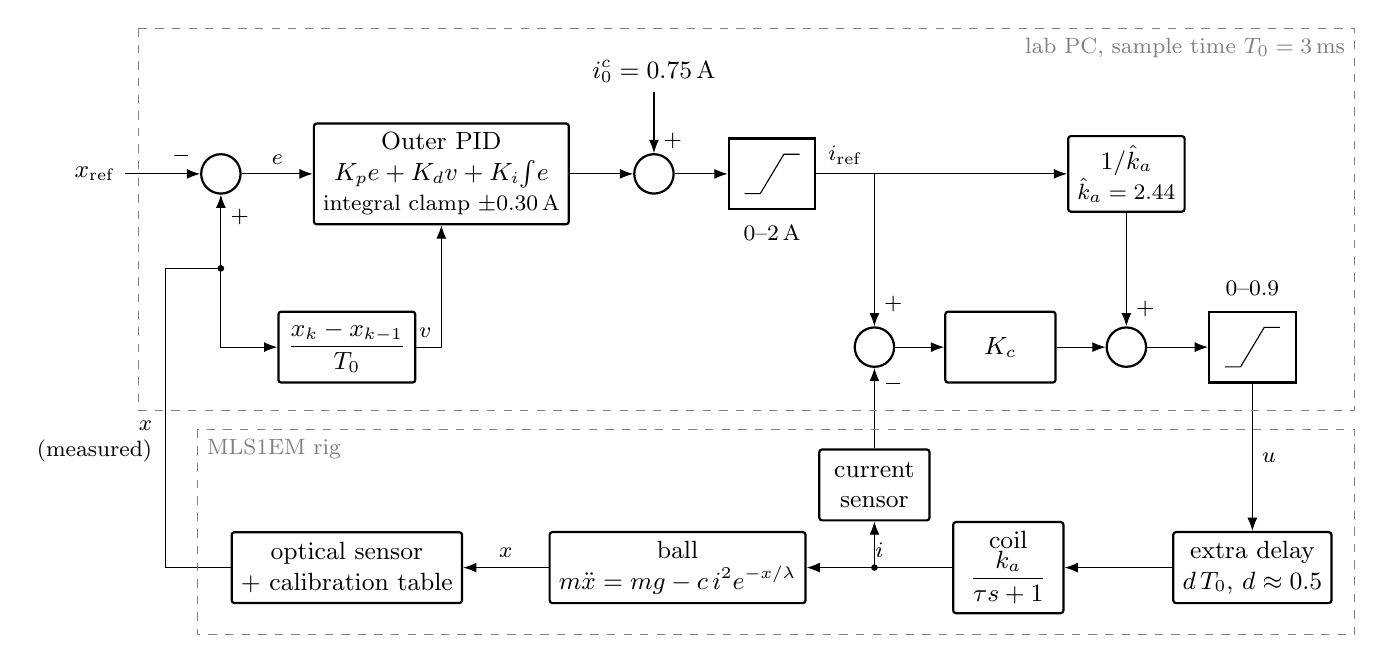
\begin{tikzpicture}[>=Latex, font=\small,
  blk/.style={draw, thick, rectangle, rounded corners=1pt, minimum height=9mm, minimum width=14mm, align=center, fill=white},
  sum/.style={draw, thick, circle, inner sep=0pt, minimum size=5mm, fill=white},
  sat/.style={draw, thick, rectangle, minimum height=9mm, minimum width=11mm, fill=white,
     path picture={\draw[thin] ([xshift=-3.5mm,yshift=-2.5mm]path picture bounding box.center) -- ([xshift=-1.5mm,yshift=-2.5mm]path picture bounding box.center) -- ([xshift=1.5mm,yshift=2.5mm]path picture bounding box.center) -- ([xshift=3.5mm,yshift=2.5mm]path picture bounding box.center);}},
  lab/.style={font=\footnotesize}]
% ---------------- controller (lab PC) ----------------
\node (xr) at (0,0) {$x_{\mathrm{ref}}$};
\node[sum] (s1) at (1.6,0) {};
\node[blk] (pid) at (4.4,0) {Outer PID\\$K_p e + K_d v + K_i\!\int\! e$\\{\footnotesize integral clamp $\pm0.30$\,A}};
\node[sum] (s2) at (7.1,0) {};
\node (i0) at (7.1,1.3) {$i_0^{c}=0.75$\,A};
\node[sat] (satI) at (8.6,0) {};
\node[lab] at (8.6,-0.75) {$0$--$2$\,A};
\coordinate (iref) at (9.9,0);
\node[sum] (s3) at (9.9,-2.2) {};
\node[blk] (kc) at (11.5,-2.2) {$K_c$};
\node[blk] (ff) at (13.1,0) {$1/\hat k_a$\\{\footnotesize $\hat k_a=2.44$}};
\node[sum] (s4) at (13.1,-2.2) {};
\node[sat] (satU) at (14.7,-2.2) {};
\node[lab] at (14.7,-1.45) {$0$--$0.9$};
\node[blk] (vel) at (3.2,-2.2) {$\dfrac{x_k - x_{k-1}}{T_0}$};
% ---------------- rig ----------------
\node[blk] (dly) at (14.7,-5.0) {extra delay\\$d\,T_0$, $d\approx0.5$};
\node[blk] (coil) at (11.6,-5.0) {coil\\$\dfrac{k_a}{\tau s+1}$};
\node[blk] (ball) at (7.4,-5.0) {ball\\$m\ddot x = mg - c\,i^2e^{-x/\lambda}$};
\node[blk] (psens) at (3.2,-5.0) {optical sensor\\+ calibration table};
\node[blk] (isens) at (9.9,-3.95) {current\\sensor};
% ---------------- wires ----------------
\draw[->] (xr) -- node[pos=0.75,above,lab]{$-$} (s1);
\draw[->] (s1) -- node[above,lab]{$e$} (pid);
\draw[->] (pid) -- (s2);
\draw[->] (i0) -- node[pos=0.8,right,lab]{$+$} (s2);
\draw[->] (s2) -- (satI);
\draw (satI) -- node[above,lab]{$i_{\mathrm{ref}}$} (iref);
\draw[->] (iref) -- (ff);
\draw[->] (iref) -- node[pos=0.85,right,lab]{$+$} (s3);
\draw[->] (s3) -- (kc);
\draw[->] (kc) -- (s4);
\draw[->] (ff) -- node[pos=0.85,right,lab]{$+$} (s4);
\draw[->] (s4) -- (satU);
\draw[->] (satU) -- node[right,lab]{$u$} (dly);
\draw[->] (dly) -- (coil);
\draw[->] (coil) -- node[above,lab]{$i$} (ball);
\draw[->] (ball) -- node[above,lab]{$x$} (psens);
\fill (9.9,-5.0) circle (1.2pt);
\draw[->] (9.9,-5.0) -- (isens);
\draw[->] (isens) -- node[pos=0.8,right,lab]{$-$} (s3);
\draw (psens.west) -- (0.9,-5.0) -- (0.9,-1.2) coordinate (xm);
\draw[->] (xm) -- (1.6,-1.2) -- node[pos=0.7,right,lab]{$+$} (s1);
\fill (1.6,-1.2) circle (1.2pt);
\draw[->] (1.6,-1.2) -- (1.6,-2.2) -- (vel);
\draw[->] (vel) -- node[above,lab,pos=0.35]{$v$} (4.4,-2.2) -- (pid);
\node[lab, anchor=east, align=right] at (0.85,-3.4) {$x$\\(measured)};
% ---------------- regions ----------------
\draw[dashed, gray] (0.55,1.85) rectangle (16.0,-3.0);
\node[gray, anchor=north east, font=\footnotesize] at (16.0,1.85) {lab PC, sample time $T_0=3$\,ms};
\draw[dashed, gray] (1.3,-3.25) rectangle (16.0,-5.85);
\node[gray, anchor=north west, font=\footnotesize] at (1.3,-3.25) {MLS1EM rig};
\end{tikzpicture}}
\caption{The cascade control loop as deployed. The outer PID turns the position error $e=x-x_{\mathrm{ref}}$ and the
velocity $v$ into a current reference; the inner loop (feed-forward $1/\hat k_a$ plus $K_c$ on the current error) makes
the coil current follow it. Gap $x$ is measured downward from the magnet; positive gains raise the current when the ball
is too low. Limits: integral contribution $\pm0.30$\,A, $i_{\mathrm{ref}}$ $0$--$2$\,A, $u$ $0$--$0.9$.}
\label{fig:blockdiag}
\end{figure}

\subsection{Experimental Setup}
\label{sec:photo}
\begin{figure}[H]\centering
\begin{subfigure}{0.56\linewidth}\centering
\figbox{../data/lab_2026-11-16/screenshots/01_rig_front_panel_photo.jpeg}{\linewidth}{5cm}
\caption{Rig and interface box}\label{fig:rig-a}
\end{subfigure}\hfill
\begin{subfigure}{0.42\linewidth}\centering
\figbox{../data/lab_2026-11-12/screenshots/00_rig_photo_calibration_stand.jpeg}{\linewidth}{5cm}
\caption{Ball resting on the calibration stand}\label{fig:rig-b}
\end{subfigure}
\caption{The INTECO MLS1EM magnetic levitation rig.}
\label{fig:rig}
\end{figure}

\subsection{Lab Models and Signal Chain}
\label{sec:labmodels}
The lab PC runs Simulink models in \emph{external mode}: the model is compiled for the rig's real-time target (``Build
for Monitoring''), runs at $T_0=3$\,ms with a fixed-step solver, and streams its scope signals to the PC. All models are
copies of the manual's templates; the original driver was never edited. The driver part of each model converts the
sensor voltage to a gap through a 33-point calibration table (\code{group22_sensor.mat}, points $0.7$\,mm apart, linear
interpolation; it must be loaded into the workspace before building), computes the velocity as
$v=(x_k-x_{k-1})/T_0$ without filtering, and sends the command to the coil as a 12-bit PWM duty (driver gain $4095$).
The command $u$ is therefore a duty fraction from $0$ to $1$; the scope labels it ``[V]'', which is not its unit.

The controller block of the manual's PD model was replaced by the cascade controller of Fig.~\ref{fig:blockdiag}
(\code{my_cascade_rt}, Fig.~\ref{fig:labmodel}): three inputs ($e$, $v$, $i$), two outputs ($u$, $i_{\mathrm{ref}}$), and a
manual test/run switch that either sends a constant test current reference (to check the inner loop with the ball on the
stand) or closes the full loop. The outer loop runs all the time, so while the ball rests on the stand the integral
winds up to its $+0.30$\,A clamp; the lift-off starts from that state. Further copies were built for the tests:
\begin{itemize}
\item \code{my_cascade_sweep_rt}: an automatic set-point sweep. A sweep clock integrates time only while $x<11.5$\,mm, so
      it starts at lift-off and pauses if the ball drops; it drives a lookup table (flat steps, 5\,s each)
      $11, 10.5, 10, 9.5, 9, 9.5, 10, 10.5, 11$\,mm. A switch selects this or a manual set point.
\item \code{my_cascade_kg_rt}: a gain $k_g$ multiplying the controller output before the $u$ limit (hardware gain-margin test).
\item \code{my_cascade_steps_rt}: small steps near the stand, $11.0 \to 10.8 \to 11.1 \to 10.6 \to 11.0 \to 10.5 \to 11.0$\,mm.
\item \code{my_cascade_ramp_rt}: a slow ramp $10.5 \to 11.4 \to 10.5$\,mm at $0.2$\,mm/s (linear interpolation).
\item \code{my_cascade_sine_rt}: a sine $A\sin(2\pi f t)$ added to the controller output before the $u$ limit, to measure
      the loop gain while levitating.
\item \code{my_cascade_D_rt}: variant~D (Section~\ref{sec:obs-varD}): a run switch holds the integral at zero while the
      coil is off; bias $0.85$\,A, integral clamp $\pm0.45$\,A.
\end{itemize}
Each run was saved from the scopes (``Print to Figure'', \code{.fig}) and read on the analysis PC with
\code{read_scope_fig.m}. The scope keeps every 3\,ms sample (it stores each one twice, as stairs; the reader removes the
copies). Logged signals: position, velocity, current and command on the main scope; current, $i_{\mathrm{ref}}$ and, in the
test models, $x_{\mathrm{ref}}$, the sweep clock, $k_g$ or the injected sine on a second scope.
\begin{figure}[H]\centering
\begin{subfigure}{0.49\linewidth}\centering
\figbox{../data/lab_2026-11-13/screenshots/01_cascade_top_level.png}{\linewidth}{4.5cm}
\caption{Top level of \code{my_cascade_rt}}\label{fig:labmodel-a}
\end{subfigure}\hfill
\begin{subfigure}{0.49\linewidth}\centering
\figbox{../data/lab_2026-11-13/screenshots/02_cascade_controller_inside.png}{\linewidth}{4.5cm}
\caption{Inside the cascade controller block}\label{fig:labmodel-b}
\end{subfigure}
\caption{The deployed lab model.}
\label{fig:labmodel}
\end{figure}

\subsection{Status Labels, Conventions and Settings}
\label{sec:status}
\paragraph{Status labels.} Every number in this report carries a status. \textbf{M} (measured) is a quantity read from
hardware data or a model fitted to hardware data. \textbf{S} (simulated) is the output of the group's MATLAB scripts or
Simulink simulations. \textbf{D} (derived) is obtained by calculation from stated values, including linear-model margins
and recalculations made while preparing this report. \textbf{N} (not obtained) marks a result that was required or
planned but not produced. \textbf{B} (benchmark) marks a value taken from the manual~\cite{mlsmanual}, not measured by the
group. The label follows the number, e.g.\ $0.798$\,A\st{D}. Where several numbers in one sentence share a label, it is
given once at the end.

\paragraph{Conventions.} The gap $x$ is measured downward from the magnet face (larger $x$ = lower ball). The position
error is $e = x - x_{\mathrm{ref}}$, and all controller gains are positive. The command $u$ is a duty fraction, not a
voltage; values of the manual's model (Section~\ref{sec:th-prelab}) are in volts and cannot be compared with lab gains.
The ball with the hole facing the magnet is called ``hole-up''; both balls were normally placed hole-up, and the rest
reading on the stand (Table~\ref{tab:settings}) was used to check the seating. ``39\,g'' and ``42\,g'' name the
$39.288$\,g and $42.137$\,g balls.

\paragraph{Three nominal points.} Three operating points appear, each for its purpose: the controller was \emph{designed}
for a bias current of $0.75$\,A, which the fitted force law gives at about $9.3$\,mm for the 39\,g ball; the
\emph{analysis} nominal (linear model, robustness, simulation cases, sine injection) is the 39\,g ball at $10$\,mm; and the
\emph{manual comparison} (Section~\ref{sec:th-prelab}) is at $9$\,mm, as in the manual.

\paragraph{Two plant fits.} The force law was fitted twice on 13 November (Section~\ref{sec:obs-ident}). ``The model''
means the combined fit ($\lambda=5.90$\,mm, 42 hover visits), used for the linear model, the robustness analysis and the
Simulink cases. The step-overshoot comparisons use the morning fit ($\lambda=5.81$\,mm, 18 visits), because they were set up
before the afternoon data existed; the two differ by $1.6\,\%$ in $\lambda$, and the text names the fit where it matters.

\paragraph{Two lift-off times.} ``Lift-off time'' is measured from the switch-on in two ways: until the reading falls
$0.2$\,mm below the rest reading (first levitation, variant~D), or until the sweep clock starts, i.e.\ until $x<11.5$\,mm
($12.0$\,mm on the lowered stand; sweeps, small steps). Times are compared only within one definition.

\begin{table}[H]
\centering
\caption{Settings of the lab models and runs}
\label{tab:settings}
\begin{tabularx}{\linewidth}{@{}>{\raggedright\arraybackslash}p{3.8cm}X@{}}
\toprule
Item & Value \\
\midrule
Sample time, solver & $T_0=3$\,ms, fixed step (\code{ode3}), external mode \\
Position measurement & 33-point calibration table, linear interpolation; driver limits $0$--$0.02$\,m \\
Velocity & $(x_k-x_{k-1})/T_0$, unfiltered \\
Command & PWM duty fraction $u$, limited to $0$--$0.9$ by the controller \\
Inner loop & $K_c = 2.05$\,/A, feed-forward $1/\hat k_a$ with $\hat k_a = 2.44$\,A per unit \\
Outer loop & $K_p = 151.2$\,A/m, $K_d = 2.6$\,A\,s/m, $K_i = 734$\,A/(m\,s), bias $i_0^c = 0.75$\,A \\
Limits & integral contribution $\pm0.30$\,A, $i_{\mathrm{ref}}$ $0$--$2$\,A \\
Variant~D & bias $0.85$\,A, integral clamp $\pm0.45$\,A, integral held at $0$ while the coil is off \\
Set points & $9$--$11$\,mm in $0.5$\,mm steps; $11.5$\,mm holds as tests only \\
Stand (rest reading) & normal $11.78$--$12.00$\,mm for hole-up seatings (39\,g hole-up $11.92$\,mm); lowered $13.13$--$13.19$\,mm \\
Recording & scope ``Print to Figure'' \code{.fig}, every $3$\,ms sample; coil-off tail after each run to measure the current-sensor zero \\
\bottomrule
\end{tabularx}
\end{table}

\subsection{Analysis Scripts and Data Files}
\label{sec:scripts}
All analysis is done by MATLAB scripts named \code{sNN_*.m}, run in order, each reading the saved lab records or the
results of earlier scripts. Every script checks itself: it prints PASS or FAIL lines for physical sanity checks, sign
tests (a controller with the wrong sign must fail) and agreement with independent calculations. A FAIL is kept when it
reports a real finding (for example, a target that was missed) and is explained where the result is used. Shared
functions provide the parameters (\code{maglev_params}), the equilibrium and linearization (\code{maglev_equilibrium},
\code{maglev_plant}), the fitted plant and uncertainty cases (\code{maglev_cases}), an independent MATLAB simulation
(\code{maglev_cascade_sim}), the Simulink model builder (\code{build_maglev_cl_sim}) and the scope-file reader
(\code{read_scope_fig}). For this report all eighteen analysis scripts were re-run on 17 November 2026; every PASS/FAIL total
matched the earlier runs and every saved result was numerically identical. Appendix~\ref{app:scripts} lists each script,
its purpose and its totals.

% ======================== 5 EXPERIMENTAL PROCEDURE ========================
\section{Experimental Procedure}
\label{sec:procedure}

\subsection{Session 1 (12 November): Discovery and Open-Loop Tests}
\label{sec:proc-1}
Ball: 39\,g. Goal: find out how the lab loop is really built, and measure the coil.
\begin{enumerate}
\item Before any run: switch on the rig's power supply, load the sensor calibration table into the workspace, work only
      on copies of the manual's example models, and build them for monitoring (never stand-alone).
\item Inspect the three example models read-only with a script (\code{s03_lab_discovery}, run on the lab PC): sample time,
      solver, filter blocks, velocity signal, controller gains and limits.
\item Try the manual's PD model. With the ball on the stand above the set point, or with the stand at $11.8$\,mm, the ball
      did not lift; the stand was then lowered and the PD gains raised ($K_p=45$) and the bias $u_0$ stepped up while running
      (run~4). The ball lifted and oscillated, hitting the stand every cycle.
\item Open-loop coil tests with the driver model: constant commands $u=0.3$, $0.6$, $1.0$, then steps
      $0 \to 0.2 \to 0.3 \to 0.4 \to 0.2$ with the ball resting on the stand at $12.9$\,mm, recording $u$ and $i$.
\end{enumerate}
After the session the cascade controller was designed offline (Section~\ref{sec:obs-design}) and checked in simulation
before it was deployed.

\subsection{Session 2 (13 November): First Levitation, Experiments A--C, Sweeps and Holds}
\label{sec:proc-2}
Balls: 39\,g and 42\,g. Goal: first levitation, identification data over the operating range, and a gain-margin test.
\begin{enumerate}
\item Build \code{my_cascade_rt} (Fig.~\ref{fig:labmodel}) and check its wiring against the design. Runs~1--2 gave no coil
      current at all: the rig's power supply was off. It was switched on.
\item Run~3, inner loop only: ball on the stand, test current reference $0.3$ then $0.5$\,A.
\item Run~4, first levitation: set point $11$\,mm, switch the loop on, let the ball lift; then step the set point to $10$\,mm.
\item Experiment~A: 39\,g ball, set point typed by hand in $0.5$\,mm steps from $11$\,mm down to $9.5$\,mm and back up to
      $11.5$\,mm.
      Experiment~B: 42\,g ball, two runs with a step $11 \to 10$\,mm, then a sweep $11 \to 9 \to 10.5$\,mm. Experiment~C: 39\,g
      ball at $10$\,mm with a gain $k_g$ on the command (\code{my_cascade_kg_rt}), stepped through
      $1, 0.8, 0.6, 0.5, 0.4, 1, 1.25, 1.5, 2, 1$.
\item Afternoon, automatic sweeps (\code{my_cascade_sweep_rt}, $11 \to 9 \to 11$\,mm): 39\,g placed hole-up, 42\,g placed
      hole-up, 42\,g placed hole-down. Then $11.5$\,mm holds (manual set point): 39\,g hole-up, 42\,g hole-up, 39\,g hole-down.
\item For every run: note the rest reading on the stand before switch-on (a seating check), and keep recording a few seconds
      after switch-off so that the current reading at $u=0$ (the current-sensor zero) can be measured.
\end{enumerate}
No log sheet was kept on this day; the set points were rebuilt from the recorded data. One more run, meant as a lift-off
from a lowered stand, had a rest reading of only $12.00$\,mm and is excluded from all analysis.

\subsection{Session 3 (16 November): Stand Tests, Sine Injection and Variant D}
\label{sec:proc-3}
Ball: 39\,g (42\,g for one run). Goal: find out why the model misfits near the stand, measure the loop gain while
levitating, and test the improved start-up (variant~D).
\begin{enumerate}
\item The rig did not respond at first: Windows did not recognize the RT-DAC/USB2 board. It was reconnected.
\item Set the stand so that the 39\,g ball (hole-up) rests at $11.87$--$12.00$\,mm, using the driver model with the command at
      $0$.
\item Small steps near the stand (\code{my_cascade_steps_rt}), 39\,g and 42\,g: $11.0 \to 10.8 \to 11.1 \to 10.6 \to 11.0 \to 10.5
      \to 11.0$\,mm, 5\,s each.
\item Slow ramp (\code{my_cascade_ramp_rt}): $10.5 \to 11.4 \to 10.5$\,mm at $0.2$\,mm/s. The first attempt ran with jumps
      instead of a ramp, because the change to linear interpolation was not in the deployed build; it was rebuilt and repeated.
\item Sine injection (\code{my_cascade_sine_rt}), 39\,g at $10$\,mm: a sine added to the command at $1.5$, $2$, $2.4$, $3$, $4$,
      $6$, $8$, $12$, $20$ and $40$\,Hz, amplitude $0.01$ (raised to $0.02$, $0.04$ and $0.08$ at $12$, $20$ and $40$\,Hz, after
      a lower-amplitude segment).
\item Lowered stand (rest reading $13.13$ and $13.19$\,mm): one run with set-point jumps up to $11.6$\,mm, and the standard
      sweep $11 \to 9 \to 11$\,mm followed by a hold at $11.5$\,mm.
\item Variant~D (\code{my_cascade_D_rt}), 39\,g on the normal stand: switch the loop on and off twice (two lift-offs), set
      point $11$\,mm with typed steps to $10.5$\,mm and back.
\end{enumerate}
Not done for lack of time: variant~D from the lowered stand, sine injection at $11$\,mm and with the 42\,g ball, and a static
sensor check with the stand moved in small steps (dropped).

\subsection{Offline Analysis and Simulation}
\label{sec:proc-offline}
The offline work ran alongside the sessions; Table~\ref{tab:scripts} gives the script for each step.
\begin{enumerate}
\item Pre-lab: reproduce the manual's model and predict the behaviour of a PD loop (s01, s02).
\item After session~1: design the cascade controller on the best model then available and check it on a grid of plants
      and in nonlinear lift-off simulations (s05).
\item After session~2: analyse the first levitation (s06); fit the force law, the coil gain and the sensor noise from the
      hover data (s07, s08); estimate the extra loop delay (s12); build the linear model and the uncertainty set (s10).
\item Check robust stability over the set (s11) and run the Simulink model over the nominal and uncertain cases in the
      hardware scenario (s09).
\item Compare simulation and hardware and investigate the misfits (s13, s14); after session~3, analyse the new tests (s16,
      s17, s18) and the follow-up questions (s19, s20, s21).
\end{enumerate}
Each script prints its own PASS/FAIL checks (Section~\ref{sec:scripts}). On 16 November all results were audited
line by line, the problems found were fixed, and the affected scripts were re-run. For this report everything was run
once more from the saved data.

% =================== 6 OBSERVATION AND DATA RECORDING ===================
\section{Observation and Data Recording}
\label{sec:obs}

\subsection{Lab Discovery and the Actuator}
\label{sec:obs-discovery}
\paragraph{The lab loop.} The inspection of the example models showed a loop different from the manual's
description\st{M}: sample time $T_0=3$\,ms (fixed step, \code{ode3}) instead of $10$\,ms; no filter blocks in the signal path;
velocity computed as the unfiltered difference $(x_k-x_{k-1})/T_0$; error convention $e = x - x_{\mathrm{ref}}$, as in the
manual. The example PD controller had $K_p = 35$, a gain of $450$ on the error difference $e_k - e_{k-1}$, and a bias
$u_0 = 0.282$; the example PID had $P=40$, $I=40$, $D=2$ and $U_0 = 0.344$.

\paragraph{First PD attempts.} With the ball resting on the stand above the set point (reading $8.4$\,mm, set point
$10$\,mm) the PD lowered the command and the ball stayed on the stand. With the stand at $11.8$\,mm the command settled at
$0.345$ and the current at $0.87$\,A, too little to lift the 39\,g ball\st{M}: the example gains are tuned for a lighter ball.
With $K_p$ raised to $45$ and the bias raised while running, the ball lifted but went into a sustained oscillation at
$7.3$--$9.3$\,Hz, $2$ to $9$\,mm peak to peak, hitting the stand every cycle (run~4\st{M}). On the linear model of the rig
built later, this PD sits on the stability boundary (Section~\ref{sec:discussion}); the large cycle itself was nonlinear.

\paragraph{Coil.} Constant commands $u = 0.3$, $0.6$, $1.0$ gave about $0.68$, $1.40$ and $2.45$\,A\st{M}
(Fig.~\ref{fig:a-coil}). In the step test with the ball on the stand at $12.9$\,mm, $u = 0.2$, $0.3$, $0.4$ gave
$0.44$, $0.69$ and $0.93$\,A\st{M}: an incremental gain of $2.33$--$2.46$\,A per unit, lower ($1.9$) for the first step from
$u=0$. The current followed each step as a first-order lag with $\tau = 22.5$--$25$\,ms while the ball rested on the
stand; after the ball jumped to the magnet at $u=0.4$ ($0.93$\,A; it did not jump at $0.69$\,A), the fitted lag was
$25$--$29$\,ms\st{M}. The manual's coil time constant, $0.63$\,ms, is therefore far too fast for this rig. The static gain
used in the model, $k_a = 2.43$\,A per unit\st{M}, was later fitted from the hover data (command against true current);
the controller's feed-forward uses $\hat k_a = 2.44$, the value available at design time.

\subsection{Identification: Force Law, Loop Delay and Sensor Noise}
\label{sec:obs-ident}
\paragraph{Current-sensor zero.} The current reading is not zero when the coil is off: at the start of a session it read
$0.03$--$0.06$\,A at $u=0$, and this offset fell by $0.3$--$1.2$\,mA per second of coil-on time, reaching $-0.02$\,A late on
16 November\st{M}. On 13 November it fell from $0.0405$ to $0.0102$\,A during the 61\,s of Experiment~A\st{M}. The true
current is therefore the reading minus a drifting zero, measured at $u=0$ before and after each run and interpolated
linearly in coil-on time. This correction matters: two visits to the same gap in one run differed by $12.0$\,mA rms in the
raw readings and by $4.8$\,mA rms after correction\st{M}. Runs without a coil-off record use the drift rate of a
neighbouring run with the same ball, or the mean rate of the session.

\paragraph{Force law.} At each hover plateau the ball is in equilibrium, so the true current and the gap give one
point of \eqref{eq:hover}. A least-squares fit of \eqref{eq:hover} to these points, with one decay length $\lambda$ for both
balls and one constant $c$ per ball, gives the force law. It was fitted twice (Table~\ref{tab:forcefit}): on the 18
morning visits, and on all 42 visits of 13 November at $9$--$11$\,mm. Plateaus with oscillation in the $1.5$--$3.5$\,Hz band
and the $11.5$\,mm holds were left out (Section~\ref{sec:obs-stand} explains why). The combined fit is the reference
model of this report (Fig.~\ref{fig:forcefit}).

\begin{table}[H]
\centering
\caption{Force-law fits $F = c\,i^2e^{-x/\lambda}$ from the hover data of 13 November}
\label{tab:forcefit}
\begin{tabular}{@{}lccc@{}}
\toprule
 & Morning fit & Combined fit (reference) & Manual \\
\midrule
Hover visits used & 18 & 42 & -- \\
$\lambda$ [mm] & 5.81 & 5.90 & 5.82 \\
$c$, 39\,g / 42\,g [N/A$^2$] & 3.37 / 3.16 & 3.29 / 3.02 & 3.01 \\
Residual [mA rms] (max) & 4.9 (10.2) & 5.9 (14.4) & -- \\
Status & M & M & B \\
\bottomrule
\end{tabular}
\end{table}

$\lambda$ is known to about $\pm0.15$\,mm; this uncertainty is systematic, because it depends on how the current zero is
modelled. The manual's $5.82$\,mm lies within it. The statistical $95\,\%$ interval of the combined fit is $\pm4.3\,\%$ for
$\lambda$ and $\pm7.4\,\%$ for $c$, but $c$ and $\lambda$ are almost perfectly correlated (correlation $-1.00$): a larger
$\lambda$ is compensated by a smaller $c$. What the linear model needs is the hover current at the operating gap, and that
is known to $\pm0.57\,\%$ over $9$--$11$\,mm\st{D}. Three further checks support the law:
\begin{itemize}
\item \emph{Prediction.} The morning law, never fitted at $9$\,mm with the 39\,g ball, predicted all 27 afternoon plateaus
      within $10.2$\,mA rms, and the 39\,g ball at $9$\,mm within $6$\,mA ($0.728$\,A measured, $0.734$\,A predicted)\st{M}.
\item \emph{Manual model.} With the manual's constants the 39\,g ball would need $0.845$\,A at $10$\,mm, $5.6\,\%$ more than
      the $0.800$\,A of the morning fit\st{D}.
\item \emph{Two balls.} The 42\,g ball needs $8.1\,\%$ more current than the 39\,g ball at the same gap, while the mass ratio
      alone explains $3.6\,\%$\st{M}; the two balls differ in size and shape (Table~\ref{tab:apparatus}), so they get separate
      $c$ values.
\end{itemize}

\repfig{forcefit}{../figs/p5_force_fit_all.png}{0.75\linewidth}{Identified force law: drift-corrected hover current
against gap for both balls, 42 visits on 13 November (morning: open circles; afternoon sweeps: filled squares), and the
combined fit $\lambda = 5.90$\,mm\st{M}. The $11.5$\,mm holds (crosses) were not fitted: they lie $0.4$--$0.5$\,mm above the
stand, where the stand-proximity effect acts (Section~\ref{sec:obs-stand}).}

\paragraph{Extra loop delay.} In run~3 (inner loop only, ball on the stand) the command $u$ and the current $i$ are logged in
the same sample: the inner-loop law \eqref{eq:inner} holds exactly at lag~0 ($R^2 = 0.9996$) and not at lags $\pm1$. A delay
between logged $u$ and $i$ is therefore a real delay in the loop. Two methods estimate it (Fig.~\ref{fig:delay}):
(A) simulate the coil from the logged command for each candidate delay and pick the best fit to the logged current:
$d = 0.55$ sample, with a $95\,\%$ interval of $0.50$--$0.55$ that is too narrow because it assumes the coil model is
exact; (B) compare the spectrum of the current noise with the loop closed and
open with the predicted noise shaping $|S|^2$ of the inner loop: $d = 0.50$, and $0.32$--$0.50$ over the coil's uncertainty
range\st{M}. Both methods reject $d=0$ and $d=1$. The open-loop coil steps of session~1 cannot tell the delays apart: away from
the first step every $d$ from $0$ to $0.75$ fits within $0.5\,\%$. The sine injection of session~3, taken while levitating,
independently supports $d \approx 0.5$--$0.6$ (Section~\ref{sec:obs-simlab}). The model uses $d = 0.5$ sample ($1.5$\,ms) as
nominal and $0.3$--$0.6$ as its range: the measured $0.32$--$0.55$ rounded outward to tenths, so that the Simulink model can
apply it exactly.

\repfig{delay}{../figs/p9_delay.png}{0.85\linewidth}{Extra loop delay from run~3\st{M}. (A) Output-error fit of the
coil model against the delay: minimum at $d = 0.55$; the open-loop coil steps are almost flat in $d$. (B) Noise shaping by the
inner loop: only a fractional delay ($d \approx 0.5$) reproduces the measured resonance near 65\,Hz. Bottom: the $0.3 \to 0.5$\,A
step with models for $d = 0$, $0.55$ and $1$.}

\paragraph{Sensor noise.} With the ball resting on the stand and $u = 0$, the readings fluctuate with standard
deviations of $0.011$\,mm (position) and $0.021$\,A (current)\st{M}. These values are used in the noisy simulation cases
(Section~\ref{sec:obs-cases}).

\begin{table}[H]
\centering
\caption{Identified parameters (reference values)}
\label{tab:identified}
\begin{tabularx}{\linewidth}{@{}>{\raggedright\arraybackslash}p{4.0cm}>{\raggedright\arraybackslash}p{4.6cm}cX@{}}
\toprule
Parameter & Value & St. & From \\
\midrule
Force decay length $\lambda$ & $5.90 \pm 0.15$\,mm & M & 42 hover visits \\
Force constant $c$ & $3.29$ / $3.02$\,N/A$^2$ (39 / 42\,g) & M & 42 hover visits \\
Coil static gain $k_a$ & $2.43$\,A per unit ($1.9$ near $u=0$) & M & hover data; coil steps \\
Coil time constant $\tau$ & $22$--$25$\,ms (model nominal $27$\,ms) & M & coil steps; sine injection \\
Extra loop delay $d$ & $0.5$ sample ($0.32$--$0.55$ measured) & M & run~3, two methods \\
Sensor noise (std) & $x$: $0.011$\,mm, $i$: $0.021$\,A & M & ball on the stand \\
Current-sensor zero & $0.03$--$0.06$\,A, falling $0.3$--$1.2$\,mA/s & M & coil-off records \\
\bottomrule
\end{tabularx}
\end{table}

\subsection{Linear Model and Uncertainty Set}
\label{sec:obs-unc}
\paragraph{Operating points.} With the identified law, \eqref{eq:hover} and \eqref{eq:lin} give the operating points of
Table~\ref{tab:oppoints}. $a_{21} = g/\lambda = 1661\,\text{s}^{-2}$ is the same at every point (unstable pole $6.49$\,Hz);
only $b$ changes, from $20.90$ to $26.77\,\text{m\,s}^{-2}\text{A}^{-1}$ over $9$--$11$\,mm and both balls ($-15$/$+9\,\%$ of the
nominal $24.59$)\st{D}. At the nominal point (39\,g, $10$\,mm, $\tau = 27$\,ms) the transfer functions \eqref{eq:tf} are
\begin{equation}
G_{xi}(s) = \frac{-24.59}{s^2 - 1661.4}\ \ \frac{\text{m}}{\text{A}}, \qquad
G_{iu}(s) = \frac{2.432}{0.027\,s + 1}\ \ \frac{\text{A}}{\text{unit}} \quad\text{(D)}.
\label{eq:tfnom}
\end{equation}

\begin{table}[H]
\centering
\caption{Operating points and linear coefficients (identified law; $a_{21}=1661\,\text{s}^{-2}$ everywhere)\st{D}}
\label{tab:oppoints}
\begin{tabular}{@{}c|ccc|ccc@{}}
\toprule
 & \multicolumn{3}{c|}{39\,g ball} & \multicolumn{3}{c}{42\,g ball} \\
$x_0$ [mm] & $i_0$ [A] & $u_0$ & $b$ [m\,s$^{-2}$A$^{-1}$] & $i_0$ [A] & $u_0$ & $b$ [m\,s$^{-2}$A$^{-1}$] \\
\midrule
9.0  & 0.733 & 0.301 & 26.77 & 0.792 & 0.326 & 24.76 \\
9.5  & 0.765 & 0.314 & 25.66 & 0.827 & 0.340 & 23.73 \\
10.0 & 0.798 & 0.328 & 24.59 & 0.862 & 0.355 & 22.75 \\
10.5 & 0.832 & 0.342 & 23.57 & 0.900 & 0.370 & 21.81 \\
11.0 & 0.868 & 0.357 & 22.60 & 0.939 & 0.386 & 20.90 \\
\bottomrule
\end{tabular}
\end{table}

\paragraph{Validity of the linearization.} The linear model was checked against the nonlinear one: its matrices agree with
a numerical Jacobian at all operating points, and it predicts the response to a small current pulse with the right sign and
size. Along all 24 simulated set-point steps of 13 November the force error of the local linearization stays below
$1.17\,\%$ of the weight; the linear and nonlinear step overshoots agree within $0.026$\,mm rms, and a single linear model
(39\,g, $10$\,mm) for both balls and all gaps within $0.086$\,mm rms\st{S} (Fig.~\ref{fig:a-linnl}). Linearization is therefore
not the cause of the lab-versus-model differences discussed in Section~\ref{sec:obs-simlab}.

\paragraph{Uncertainty set.} Table~\ref{tab:uncset} lists the parameters that vary, their ranges and the evidence. Each
range covers the measured values with some margin. Every combination of the extreme and middle values forms a grid of
$1458$ plants (2 balls $\times$ 3 gaps $\times$ 3 values each of $\lambda$, $c$, $\tau$, $k_a$ and $d$). Mapped onto the linear model,
the set spans $a_{21} = 1582$--$1749\,\text{s}^{-2}$ (unstable pole $6.33$--$6.66$\,Hz) and $b = 19.40$--$28.44\,\text{m\,s}^{-2}\text{A}^{-1}$
($-21$/$+16\,\%$)\st{D}. As a check, every one of the 42 measured hover currents lies inside the band of currents the set
predicts, the closest $35.9$\,mA from its edge; at $10$\,mm (39\,g) the band is $0.748$--$0.856$\,A ($-6.3$/$+7.3\,\%$),
about five times wider than the measured scatter, as intended (Fig.~\ref{fig:lincoeffs}).

\begin{table}[H]
\centering
\caption{The uncertainty set and its justification}
\label{tab:uncset}
\begin{tabularx}{\linewidth}{@{}>{\raggedright\arraybackslash}p{3.0cm}>{\raggedright\arraybackslash}p{2.6cm}>{\raggedright\arraybackslash}p{3.0cm}X@{}}
\toprule
Parameter & Nominal & Range & Evidence \\
\midrule
Ball mass $m$ & 39.288\,g & 39.288 / 42.137\,g & the two lab balls \\
Operating gap $x_0$ & 10\,mm & 9--11\,mm & validated hover range, both balls; stand $\geq 0.85$\,mm below the set point \\
Decay length $\lambda$ & 5.90\,mm & $\pm5\,\%$ (5.6--6.2\,mm) & fits 5.81 / 5.90\,mm, manual 5.82; covers the 95\,\% interval $\pm4.3\,\%$ \\
Force constant $c$ & 3.29 / 3.02\,N/A$^2$ & $\pm5\,\%$ & refits on different data moved $c$ by 2--4\,\%; residual 5.9\,mA $\approx 1.4\,\%$ of the force \\
Coil time constant $\tau$ & 27\,ms & 20--35\,ms & measured 22--25\,ms (steps, sine), up to 29\,ms with the ball at the magnet; widened for heating and gap-dependent inductance \\
Coil gain $k_a$ & 2.43\,A/unit & 2.2--2.7\,A/unit & incremental 2.33--2.46 (coil steps), 2.43 (hover data) \\
Extra delay $d$ & 0.5 sample & 0.3--0.6 sample & measured 0.32--0.55 (two methods), rounded outward \\
\midrule
\multicolumn{4}{@{}l}{\emph{Simulation cases only (not in the robust-stability grid):}} \\
Sensor noise & 0 & $x$ 0.011\,mm, $i$ 0.021\,A & readings on the stand \\
Current-zero drift & 0 & $-0.85$\,mA/s & coil-off records of the long sweeps \\
\midrule
\multicolumn{4}{@{}l}{\emph{Outside the set:}} \\
Gain error $k_g$ on $u$ & 1 & 0.4 and 2.0 & hardware gain-margin test (Experiment~C); see Section~\ref{sec:obs-robust} \\
\bottomrule
\end{tabularx}
\end{table}

The actuator gain error $k_g$ of Experiment~C is kept out of the set on purpose. Applied to the whole grid, $k_g = 0.4$ makes
some extreme corners unstable; since the hardware stayed stable at $k_g = 0.4$, the real plant is not at those corners, and
Experiment~C is a test of the nominal loop's gain margin, not a part of the uncertainty (Section~\ref{sec:obs-robust}).

\paragraph{Unmodelled effects.} Effects not in the parametric set: the stand-proximity effect (within about $0.7$--$0.8$\,mm
of the stand; Section~\ref{sec:obs-stand}), which the claimed range avoids by keeping the stand at least $0.85$\,mm below
the set point; the cause of the extra delay (its size is in the set); back-EMF and gap-dependent inductance of the coil
(small, and the inner loop rejects them); the lower coil gain near $u = 0$ (only at lift-off); the current-zero drift and the
sensor noise (simulation cases; the integral removes the drift); and the kinks of the 33-point position calibration table.
How much room the controller leaves for such effects is quantified in Section~\ref{sec:obs-robust}.

\repfig{lincoeffs}{../figs/p7_linear_coeffs.png}{0.85\linewidth}{Left: hover current against gap from the identified law,
with the 42 lab visits (dots) and the band covered by the uncertainty set (shaded); star = analysis nominal. Right: input gain
$b = 2g/i_0$; $a_{21}$ is the same at every gap\st{D}. The $11.5$\,mm region (grey) is outside the claimed range.}
\repfig{plantbode}{../figs/p7_plant_bode.png}{0.75\linewidth}{Frequency response of the plant $u \to x$ (ZOH, $T_0 = 3$\,ms):
the nominal 39\,g and 42\,g plants at $10$\,mm with $d = 0.5$ (colour) and 192 corners of the set at $d = 0.3$ and $0.6$
(grey)\st{D}. The dashed line marks the unstable pole at $6.5$\,Hz.}

\subsection{Controller Design}
\label{sec:obs-design}
\paragraph{Design model.} The controller was designed after session~1, before the force law, the delay or the hover current
were known. The design therefore used the manual's decay length ($a_{21} = g/P_2 = 1684.7\,\text{s}^{-2}$), a bias current
$i_0^c = 0.75$\,A ($b = 2g/0.75 = 26.16$), a coil with $\tau = 27$\,ms and $k_a = 2.44$\,A per unit from the coil steps, and
$T_0 = 3$\,ms with no extra delay. These differ from the later identified values by a few per cent; the robustness analysis
(Section~\ref{sec:obs-robust}) re-checks the \emph{deployed} gains against the identified set, so the design values do not
need to be exact.

\paragraph{Choices.} The inner loop was given a closed-loop time constant $\tau_{\mathrm{in}} = 3$\,ms, one sample, about nine
times faster than the coil. The outer poles were placed at $\omega_n = 40$\,rad/s with $\zeta = 0.7$ and the integral pole at
$\omega_i = 12$\,rad/s. The closed-loop pair, at $-28 \pm j28.6$\,rad/s, then has a natural frequency close to the speed of the
unstable pole ($p = 40.76$\,rad/s) and good damping, and the integral pole is slow enough not to disturb the transient. A sweep of
$\omega_n$, $\zeta$ and $\tau_{\mathrm{in}}$ against the design grid (below) preceded the choice; it found $\tau_{\mathrm{in}}=3$\,ms
best for the worst-case $M_s$. That sweep was not saved, so no numbers are quoted from it.

\paragraph{Gains.} Equations \eqref{eq:kc} and \eqref{eq:gains} give the gains of Table~\ref{tab:gains} (arithmetic in
Section~\ref{sec:calc}). They were deployed unchanged on all three lab days; a regression of the logged $i_{\mathrm{ref}}$ on
the logged error and velocity during the sweeps recovers $K_p = 151.6$\,A/m and $K_d = 2.53$\,A\,s/m\st{M}, which confirms
both the values and the sign convention on the hardware.

\begin{table}[H]
\centering
\caption{Controller gains and limits (deployed)}
\label{tab:gains}
\begin{tabular}{@{}llll@{}}
\toprule
Quantity & Design value & Deployed & Unit \\
\midrule
Inner-loop gain $K_c$ & 2.054 & 2.05 & 1/A \\
Feed-forward $1/\hat k_a$ & $1/2.44$ & $1/2.44$ & 1/A \\
$K_p$ & 151.25 & 151.2 & A/m \\
$K_d$ & 2.599 & 2.6 & A\,s/m \\
$K_i$ & 733.9 & 734 & A/(m\,s) \\
Bias $i_0^c$ & 0.75 & 0.75 & A \\
Integral clamp & $\pm0.30$ & $\pm0.30$ & A (contribution to $i_{\mathrm{ref}}$) \\
Limits & $i_{\mathrm{ref}}$ 0--2, $u$ 0--0.9 & same & A, -- \\
\bottomrule
\end{tabular}
\end{table}

\paragraph{Checks at design time.} Before the gains went to the hardware they were checked on the linear sampled loop and in
nonlinear simulation\st{S}:
\begin{itemize}
\item The nominal design loop is stable with $M_s = 1.36$. Negating all gains makes it unstable (the sign test).
\item A grid of 81 plants ($\tau$ $20$/$27$/$35$\,ms $\times$ $k_a$ $2.2$/$2.44$/$2.7$ $\times$ three force-decay lengths $\times$ $i_0$
      $0.65$/$0.75$/$0.90$\,A) is stable everywhere, with worst $M_s = 1.67$; with one extra sample of delay it is still stable,
      but the worst $M_s$ rises to $5.23$. This showed early that the loop delay matters, and it was measured on 13 November
      (Section~\ref{sec:obs-ident}). Two of the three decay lengths (8.3 and 10\,mm) came from a pre-lab reading of the stand
      lift-off thresholds that was later withdrawn; the grid was a design-time check only and is superseded by the analysis of
      Section~\ref{sec:obs-robust}.
\item The inner loop was predicted to reach $63\,\%$ of a $0.3 \to 0.5$\,A step in $3.0$\,ms, against $27$\,ms for the open coil
      (Fig.~\ref{fig:a-inner}); the lab measured 2 samples (Section~\ref{sec:obs-first}).
\item Nonlinear lift-off simulations from the stand, with the integral wound up, lifted the ball in every case without
      touching the magnet; they also used the withdrawn force constants and are shown only as a pre-lab check
      (Fig.~\ref{fig:a-liftsim}).
\end{itemize}

\subsection{First Levitation and Experiments A--C}
\label{sec:obs-first}
\todo{E}{Run 3 and run 4 (H1--H5); experiments A, B, C (I1--I9).}
\repfig{run3}{../figs/p3_lab_run3.png}{0.75\linewidth}{Run 3: measured inner current loop, ball on the stand.}
\repfig{run4}{../figs/p3_lab_run4.png}{0.85\linewidth}{Run 4: first levitation with the cascade controller.
\capnote{``simulation (Phase 3)'' uses the pre-identification plant}}
\repfig{expAB}{../figs/p4_sweep_lab_vs_sim.png}{0.85\linewidth}{Experiments A and B: gap sweeps, lab vs simulation.
\capnote{simulation with $d=0$; the set-point typo is inferred, not confirmed}}
\repfig{kgtest}{../figs/p4_kg_test.png}{0.85\linewidth}{Experiment C: actuator gain $k_g$ from 0.4 to 2.0.
\capnote{$k_g$ is a hardware gain-margin test, not part of the robust set}}

\subsection{Automatic Sweeps and \texorpdfstring{11.5\,mm}{11.5 mm} Holds}
\label{sec:obs-sweeps}
\todo{E}{Validated range (J1--J7).}
\repfig{sweeps}{../figs/p5_sweeps_lab_vs_sim.png}{0.85\linewidth}{Automatic sweeps 11--9--11\,mm, lab vs simulation.
\capnote{simulation with $d=0$, morning-fitted plant}}
\repfig{roll}{../figs/p5_42g_roll.png}{0.8\linewidth}{Lift-offs: the 42\,g ball placed hole-up rolls over.}
\repfig{hold115}{../figs/p5_hold115_rocking.png}{0.85\linewidth}{11.5\,mm holds on the normal stand: the 2.4\,Hz rocking.
\capnote{the title's ``$\sim$20$\times$'' is 14$\times$ in std and 19$\times$ in band rms}}

\subsection{Robustness Analysis}
\label{sec:obs-robust}
\todo{E}{Nominal and grid-worst margins, $M_s$ target missed, $|WT|$ options, room for unmodelled error, Exp~C trimming
(K1--K15).}
\repfig{margins}{../figs/p8_margins.png}{0.9\linewidth}{Margins over the 1458-point uncertainty grid.
\capnote{worst $M_s$ 2.23 exceeds the target 2}}
\repfig{wtopt}{../figs/p8_WT_options.png}{0.85\linewidth}{Robust stability test $|WT|<1$: one disk, Option~1, Option~2.
\capnote{Options 1 and 2 were added after the one-disk test failed}}

\subsection{Nonlinear Simulation Cases}
\label{sec:obs-cases}
\todo{E}{77 cases, 69 in the set: 51 fully OK, 18 within 0.1\,mm of the stand, none lost (L1--L8).}
\repfig{corners}{../figs/p6_cases_corners.png}{0.9\linewidth}{Simulated sweeps at the corners of the uncertainty set.
\capnote{the grey trace held at about 11.2\,mm is the clamp-limited corner (204\,\textmu m steady error)}}
\repfig{special}{../figs/p6_cases_special.png}{0.9\linewidth}{Simulated special cases.
\capnote{$k_g$ tests are outside the set; the 11.5\,mm cases are stress cases}}

\subsection{Simulation versus Hardware}
\label{sec:obs-simlab}
\todo{E}{Step overshoot (M1--M6), sine injection (P1--P6), lift-off (Q7, Q8, R1--R3).}
\repfig{mismatch}{../figs/p10_overshoot_mismatch.png}{0.9\linewidth}{Down-step overshoot mismatch and the braking spike.
\capnote{H-force curve = rejected hypothesis; panel (d) title predates the stand-tied finding}}
\repfig{sine}{../figs/p13_sine_loop.png}{0.9\linewidth}{Loop gain measured by sine injection (39\,g, 10\,mm).
\capnote{1.5--2.4\,Hz points too noisy}}

\subsection{The Stand-Proximity Effect and the \texorpdfstring{2.4\,Hz}{2.4 Hz} Rocking}
\label{sec:obs-stand}
\todo{E}{Static deficit, braking spike (11 spikes, 0.67--0.89\,mm), rocking, lowered stand, lift-off zone test
(N1--N13, O1--O7). Never ``shadowing'', never ``rotation''.}
\repfig{steps3a}{../figs/p12_3a_steps.png}{0.9\linewidth}{Small steps near the stand (16 November).}
\repfig{standprox}{../figs/p14_stand_proximity.png}{0.9\linewidth}{Braking spike vs stand position.
\capnote{the spike moves with the stand}}
\repfig{rocking}{../figs/p11_rocking.png}{0.9\linewidth}{Bounds on the 2.4\,Hz rocking.
\capnote{panel (d) ``$\geq0.19$'' holds only for an unstructured error}}
\repfig{liftzone}{../figs/p16_liftoff_stand_height.png}{0.75\linewidth}{Force factor near the stand: slow ramp vs lift-offs.
\capnote{lift-offs cross the zone too fast: they neither confirm nor refute the static effect}}

\subsection{Controller Improvement: Variant D}
\label{sec:obs-varD}
\todo{E}{Clamp/bias options in simulation; variant D on the hardware (Q1--Q8, L8, L9).}
\repfig{clampfix}{../figs/p8_clamp_fix.png}{0.85\linewidth}{Lift-off with the integral wound up: options A--D (simulation).}
\repfig{varD}{../figs/p15_variantD_ramp.png}{0.95\linewidth}{Variant D on the hardware and the slow ramp.
\capnote{$n=2$ vs 3 lift-offs, 39\,g, normal stand}}

\subsection{Practical Issues Log}
\label{sec:issues}
\todo{E}{Rig power off (13 Nov runs 1--2), USB board not recognized (16 Nov), Flat vs Linear table, missing coil-off
tails, ball seating, no log sheet on 13 Nov.}

% ============================== 7 CALCULATIONS ==============================
\section{Calculations}
\label{sec:calc}
\todo{F}{Worked examples T1--T12 of numbers.md: hover current, linear coefficients, controller gains, delay in ms, stand
deficit as a fraction of the weight, Exp~A set-point bound.}

% ================================ 8 RESULTS ================================
\section{Results}
\label{sec:results}
\todo{F}{Summary table: each requirement R1--R5 / deliverable D1--D6, the result with its status label, and where it is
shown.}

% =============================== 9 DISCUSSION ===============================
\section{Discussion}
\label{sec:discussion}
\todo{F}{Comparison with theory and simulation; why a cascade (Fig.~\ref{fig:pdgrid}); sources of error; unresolved items;
unconfirmed items stated openly (Exp~A set-point typo inferred from the data; conversion of $u$ to volts not verified);
the missed $M_s$ target; limitations.}
\repfig{pdgrid}{../figs/p17_pd_gain_grid.png}{0.95\linewidth}{Position-only PD on the linear model vs the cascade.
\capnote{best PD for all 9 corners: worst $M_s$ 10.4; cascade 1.99 at the same corners}}

% =============================== 10 CONCLUSION ===============================
\section{Conclusion}
\label{sec:conclusion}
\todo{F}{Major findings and whether the objectives were achieved.}

% =============================== 11 PRECAUTIONS ===============================
\section{Precautions}
\label{sec:precautions}
\todo{F}{Rig power and USB check; SensorData before building; Build for Monitoring; stand height and seating check;
coil-off tails; step size near the stand; verify the deployed build (Flat vs Linear); integral reset.}

% ================================ REFERENCES ================================
\begin{thebibliography}{99}

\bibitem{ps9}
Dr. Y. V. Karteek, ``Problem Statement 9: Magnetic levitation,'' \textit{EE302 Control Systems Laboratory, Final
Project}, Indian Institute of Technology Mandi, Aug.--Dec. 2026.

\bibitem{mlsmanual}
INTECO, \textit{Magnetic Levitation System MLS1EM USB2: User's Manual}, Krak\'ow, Poland.

\bibitem{ogata}
K. Ogata, \textit{Modern Control Engineering}, 5th ed. Upper Saddle River, NJ, USA: Prentice Hall, 2010.

\bibitem{franklin}
G. F. Franklin, J. D. Powell, and A. Emami-Naeini, \textit{Feedback Control of Dynamic Systems}, 8th ed. New York,
NY, USA: Pearson, 2019.

\bibitem{skogestad}
S. Skogestad and I. Postlethwaite, \textit{Multivariable Feedback Control: Analysis and Design}, 2nd ed. Chichester,
UK: Wiley, 2005.

\end{thebibliography}

% ================================ APPENDICES ================================
\clearpage
\appendix
\section{Additional Figures}
\label{app:figs}
\todo{F}{One-line context for each appendix figure.}
\repfig{a-force}{../figs/p1_force_curves.png}{0.75\linewidth}{Manual force model, 57.1\,g ball (benchmark).}
\repfig{a-sweep}{../figs/p1_sweep.png}{0.8\linewidth}{Manual model: equilibrium and linearization vs gap.
\capnote{manual model; $u$ in volts, not the duty $u$ of this report}}
\repfig{a-polemap}{../figs/p2_polemap.png}{0.85\linewidth}{Open-loop poles and zeros of the manual plant (pre-lab).}
\repfig{a-inner}{../figs/p3_inner_step.png}{0.7\linewidth}{Predicted inner-loop step response.}
\repfig{a-liftsim}{../figs/p3_liftoff_sim.png}{0.75\linewidth}{Pre-lab lift-off simulation of the cascade controller.
\capnote{pre-lab check only; force constants from a withdrawn premise}}
\repfig{a-linnl}{../figs/p7_lin_vs_nl_overshoot.png}{0.85\linewidth}{Overshoot of the 24 afternoon steps: lab, nonlinear and
linear models.}
\repfig{a-flip}{../figs/p4_42g_flip.png}{0.8\linewidth}{Experiment B: the 42\,g ball turning over after lift-off.}
\repfig{a-wt}{../figs/p8_WT.png}{0.8\linewidth}{Multiplicative uncertainty and the one-disk $|WT|$ test.}
\repfig{a-coil}{../data/lab_2026-11-12/screenshots/07_scope_coil_test_0p3_0p6_1p0.png}{0.75\linewidth}{Open-loop coil test,
$u=0.3$, 0.6, 1.0 (scope screenshot, 12 November).}
\begin{figure}[H]\centering
\begin{subfigure}{0.49\linewidth}\centering
\figbox{../data/lab_2026-11-16/screenshots/04_sine_model_top_level.png}{\linewidth}{4.5cm}
\caption{Sine-injection model}\label{fig:a-models-a}
\end{subfigure}\hfill
\begin{subfigure}{0.49\linewidth}\centering
\figbox{../data/lab_2026-11-16/screenshots/05_variantD_model_top_level.png}{\linewidth}{4.5cm}
\caption{Variant D model}\label{fig:a-models-b}
\end{subfigure}
\caption{Test models built on 16 November.}
\label{fig:a-models}
\end{figure}

\section{Scripts, Data Files and Self-Checks}
\label{app:scripts}
Totals are from the re-run of 17 November 2026 on the analysis PC (\code{matlab -batch}). ``Lab'' scripts were run only
on the lab PC or are helpers for it; they produce no results quoted here.

{\small
\begin{longtable}{@{}l>{\raggedright\arraybackslash}p{5.0cm}>{\raggedright\arraybackslash}p{1.4cm}>{\raggedright\arraybackslash}p{3.7cm}@{}}
\caption{Analysis scripts, outputs and self-check totals}\label{tab:scripts}\\
\toprule
Script & Purpose & PASS / FAIL & Meaning of a FAIL \\
\midrule
\endfirsthead
\toprule
Script & Purpose & PASS / FAIL & Meaning of a FAIL \\
\midrule
\endhead
\code{s01_verify_model} & Reproduce the manual's model numbers & 36 / 0 & -- \\
\code{s02_plant_analysis} & Pre-lab plant analysis and PD prediction (manual model) & 39 / 0 & -- \\
\code{s03_lab_discovery} & Inspect the lab models on the lab PC & lab & -- \\
\code{s04_save_scope_traces} & Save scope traces on the lab PC & lab & -- \\
\code{s05_cascade_design} & Cascade controller design and design-time grid & 28 / 0 & -- \\
\code{s06_analyze_cascade_run} & First levitation (runs 3, 4) & 7 / 0 & -- \\
\code{s07_analyze_experiments} & Experiments A, B, C; morning force-law fit & 10 / 0 & -- \\
\code{s08_analyze_sweeps} & Sweeps and 11.5\,mm holds; combined force-law fit & 21 / 0 & -- \\
\code{s09_sim_models} & Simulink model, 77 nominal and uncertain cases, variant~D & 16 / 1 & 18 cases in the set come within 0.1\,mm of the stand \\
\code{s10_linear_model} & Linear model, linearization checks, uncertainty table & 12 / 0 & -- \\
\code{s11_robustness} & Margins over the grid, $|WT|$ tests, integral clamp options & 12 / 4 & $M_s$ target missed; one-disk and Option~1 tests fail; options A--C bring the ball within 6\,mm of the magnet \\
\code{s12_delay_estimate} & Extra loop delay & 7 / 0 & -- \\
\code{s13_overshoot_mismatch} & Down-step overshoot mismatch, braking spike & 13 / 1 & a rejected hypothesis does not explain the mismatch \\
\code{s14_rocking} & 2.4\,Hz rocking & 11 / 0 & -- \\
\code{s15_rebuild_lab_models} & Backup rebuilder of the lab models & lab & -- \\
\code{s16_analyze_3a} & Small steps near the stand (16 Nov) & 9 / 2 & two runs without a coil-off tail \\
\code{s17_analyze_1116} & Sine injection, stand position, lowered-stand lift-off & 10 / 2 & one step came within 0.03\,mm of the stand; lowered-stand lift-offs outside the simulated range \\
\code{s18_analyze_D_ramp} & Variant~D on the hardware, slow ramp & 5 / 0 & -- \\
\code{s19_trim_expC} & Effect of Experiment~C on the robustness test & 5 / 0 & -- \\
\code{s20_liftoff_stand_height} & Lift-off forces by height above the stand & 6 / 0 & -- \\
\code{s21_pd_gain_grid} & Position-only PD vs the cascade & 6 / 1 & an earlier, unsaved grid result is not reproduced (this script's numbers are used) \\
\bottomrule
\end{longtable}}

\end{document}
